\section{Conception de notre algorithme}
    \subsection{Notre algorithme}
    % \begin{itemize}
    %     \item On a pris l'interaction des forces totale sur chaque particule par la fonction dans l'article `Cheerios effect'
    %     \item et de ca on deduis la force que reagis a chaque cheerios pour un pas de temps 
    %     \item Check si il ya des collisions ou pas et si il ya on change les proprietes des cheerios par rapport aux collisions
    %     \item De la force en utilisant l'integration de verlet et le principe fondamentale de la dynamique somme forces = derive (masse*vitesse) on peux changer les positions des cheerios
    % \end{itemize}
    % Pour nos calculs pour la force de interaction des objets-bords et objet-objet on a utilise lequation\ref{eq:ForceInteraction}. Le seul probleme avec cela on a besoin de savoir langle de contact de lobjet et du bords.  PAS SUR DE LE METTRE ON A DEJA TOUT DIT DE CELA.
        % Et pour nos objets flottants on a utilise \cite{lattice_boltzmann_caplilary_interaction}  PAS COMPRIS DE QUOI TU PARLES.
        Voici un diagramme du fonctionnement de notre algorithme pour un seul objet (s'il y a x objets alors on répète x-fois celui-ci). (\ref{diag:algorithme}).
        %J'ai préciser dans le titre pour un objet.
        \begin{figure}[H]
            \centering
            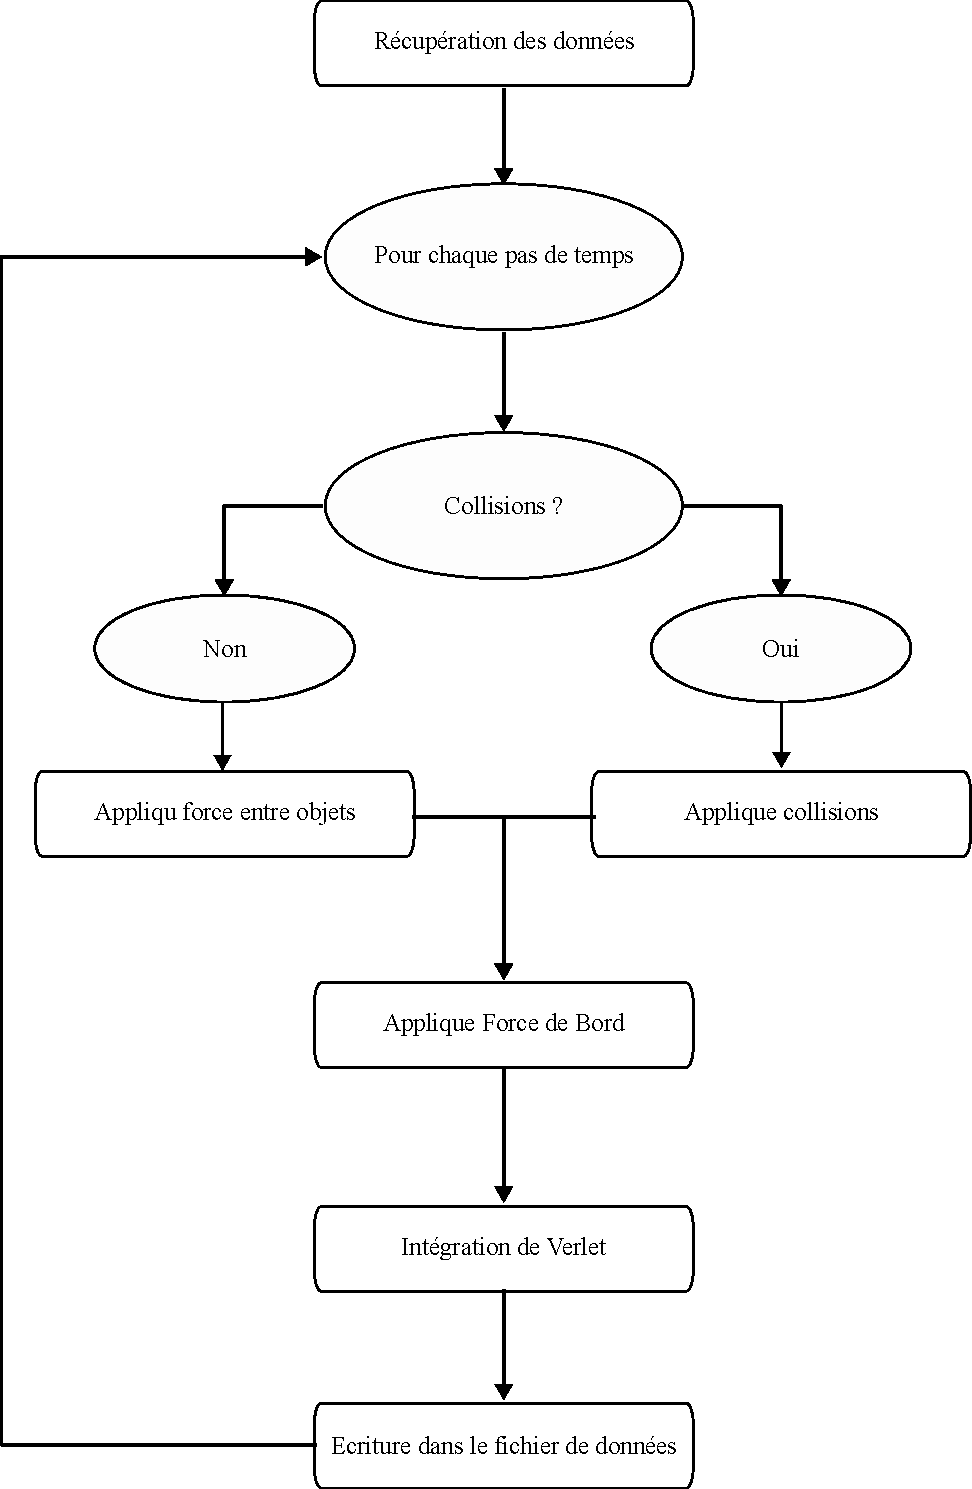
\includegraphics[width=0.45\textwidth]{Diagramme.pdf}
            \caption{Diagramme de notre algorithme pour un objet.}
            \label{diag:algorithme}
        \end{figure} 

        Nous avons essayé d'être le plus efficace dans notre programme et de limiter le nombre d'itération. Les données initiales sont à mettre dans un fichier texte, les données finales sont également mises dans un fichier texte. Ce dernier est lu par un script Python afin de créer l'animation avec matplotlib et sa classe \textit{animate}. Pour représenter nos objets nous utilisons la classe \textit{circle} de matplotlib également. Cela nous permet de définir des cercles avec des rayons précis.
    
    \subsection{Améliorations possibles}
        % \begin{itemize}
        %     \item Code en $O(NT\,n^2)$ et peux etre ameliorer en $O(NT\, n\log n)$ en faisant le calcul de collisions plus inteligament a la place de une recherche exasthive et en calculant une seule fois le \textit{millieu} des forces de chaque particule pour avoir un centre de atraction et comme ca on calcule le centre de attraction regarde si on a des collisions ou pas et a la fin ajoute les forces du bords a chaque particule
        %     \item pour linstant on utilise les equations \textit{aproximatives} on peux les essayer de les resoudres sans approximations en utilisant laproximation de Nicholson(fine difference method)
        %     \item le code marche seulement pour les objets ronds faux ajouter une facon plus complexe pour plus de objets
        % \end{itemize}
        Notre code, actuellement n'est pas optimisé pour déterminer s'il y a des collisions entre les objets. En effet, nous regardons pour chaque objet s'il est en collision avec tous les autres objets présents. Cela nous donne un algorithme qui s'effectue en $O(NT\,n^2)$ ($NT$: nombre de pas de temps total dans la simulation, $n$: nombre d'objet), alors que nous pourrions l'effectuer en $O(NT\, n\log n)$. En utilisant un algorithme plus efficace. Seule l'amélioration dans la detection des collisions ne suffirait pas, car pour calculer les forces nous aurons quand meme une complexité de  $O(n^2)$ et notre temps d'exécution de notre programme augmenterait puisque nous faisons les calculs des forces et le test des collisions en même temps. Pour atteindre une complexité plus basse, nous aurons aussi besoin d'optimiser les calculs des forces. Pour cela, nous pouvons prendre un point dans lequel nous pouvons projeter toutes les forces et pour chaque particule prendre la force entre le point où les forces sont projetées.

        Nous utilisons actuellement certaines équations qui sont approximatives, nous pourrions utiliser des équations plus précises comme l'approximation de Nicholson pour trouver un angle de contact plus précis et plus fiable.

        Enfin, notre code fonctionne uniquement avec des objets sphériques de même taille. Nous pourrons ajouter les calculs pour différentes formes géométrique.
\newpage
\onecolumn
\section{Nos Résultats}
    Pour tester notre programme nous avons fait l'expérience en vrai. Nous avons mis différents objets sphériques dans un bol rempli d'eau et nous avons filmer leurs mouvements. Nous avons ensuite analysé leurs coordonnées initiales avec Tracker et nous les avons implémentées dans notre code. Nous avons pu, après cela, analyser les différences entre la réalité et notre simulation. Voici sur les Figures suivantes nos comparaisons pour l'une d'elles.

    % \begin{figure}[H]
    %     \centering
    %     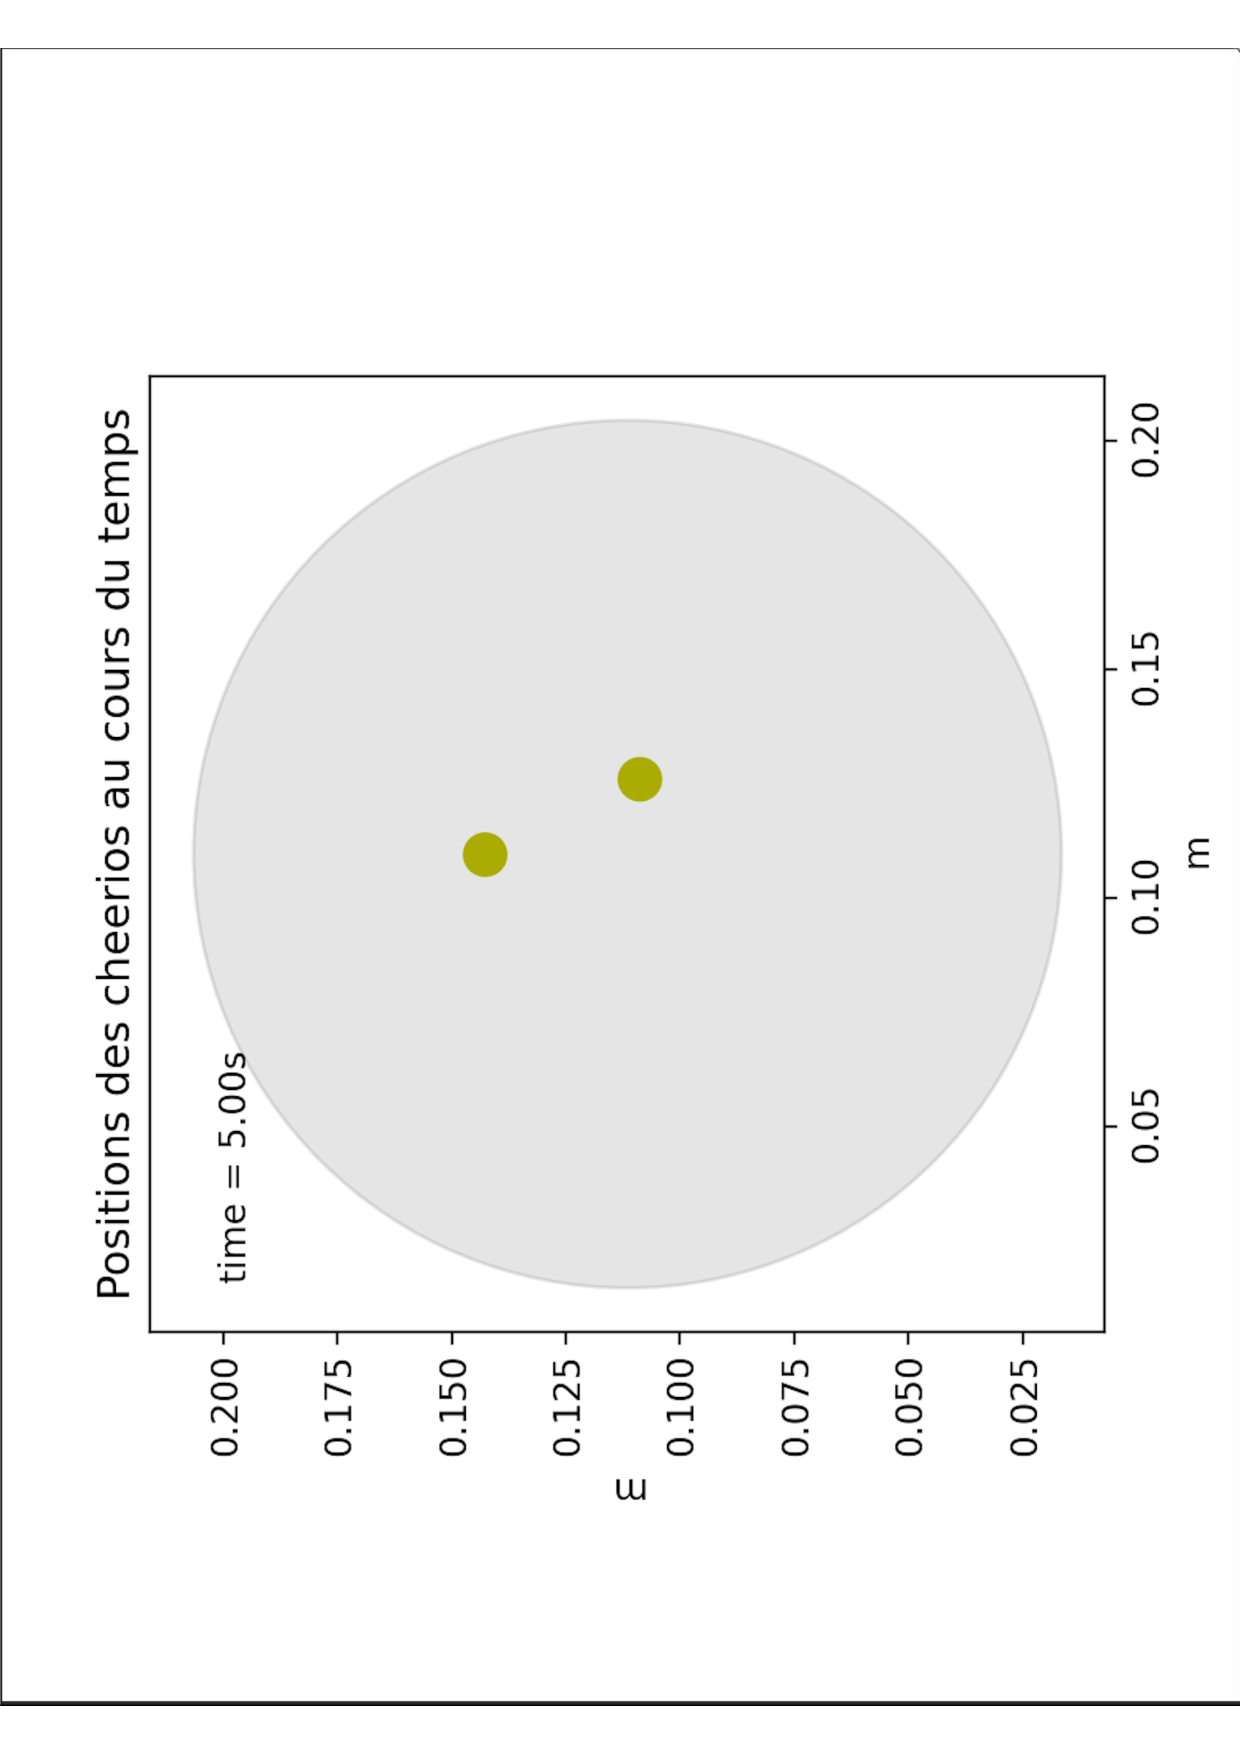
\includegraphics[width=0.4\textwidth]{visualisation3_1000_init.pdf}
    %     \caption{Image de notre simulation lorsque les objets sont à leurs positions originales}
    %     \label{fig:simul_init}
    % \end{figure}
    % \begin{figure}[H]
    %     \centering
    %     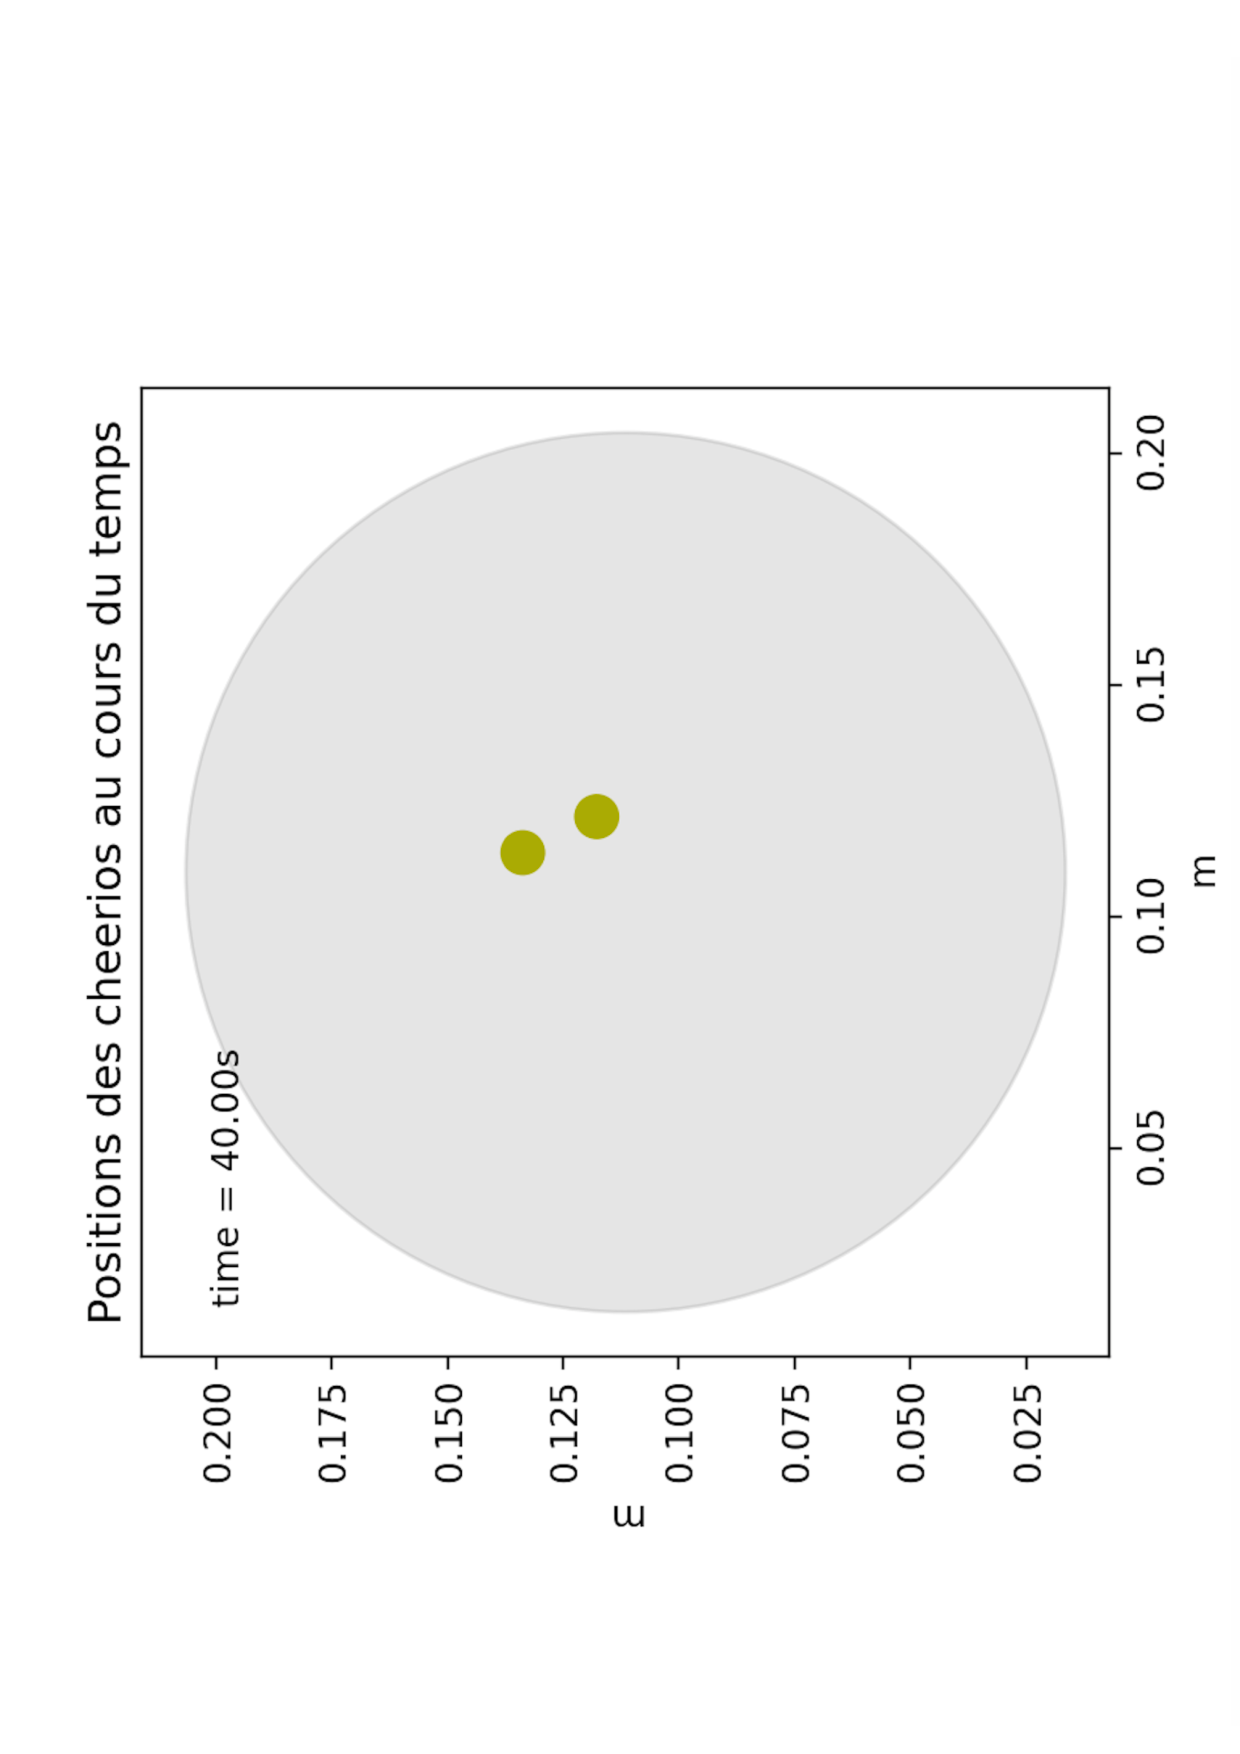
\includegraphics[width=0.4\textwidth, angle = 270]{visualisation3_1000_pres.pdf}
    %     \caption{Image de notre simulation lorsque les objets sont proches}
    %     \label{fig:simul_pres}
    % \end{figure}
    % \begin{figure}[H]
    %     \centering
    %     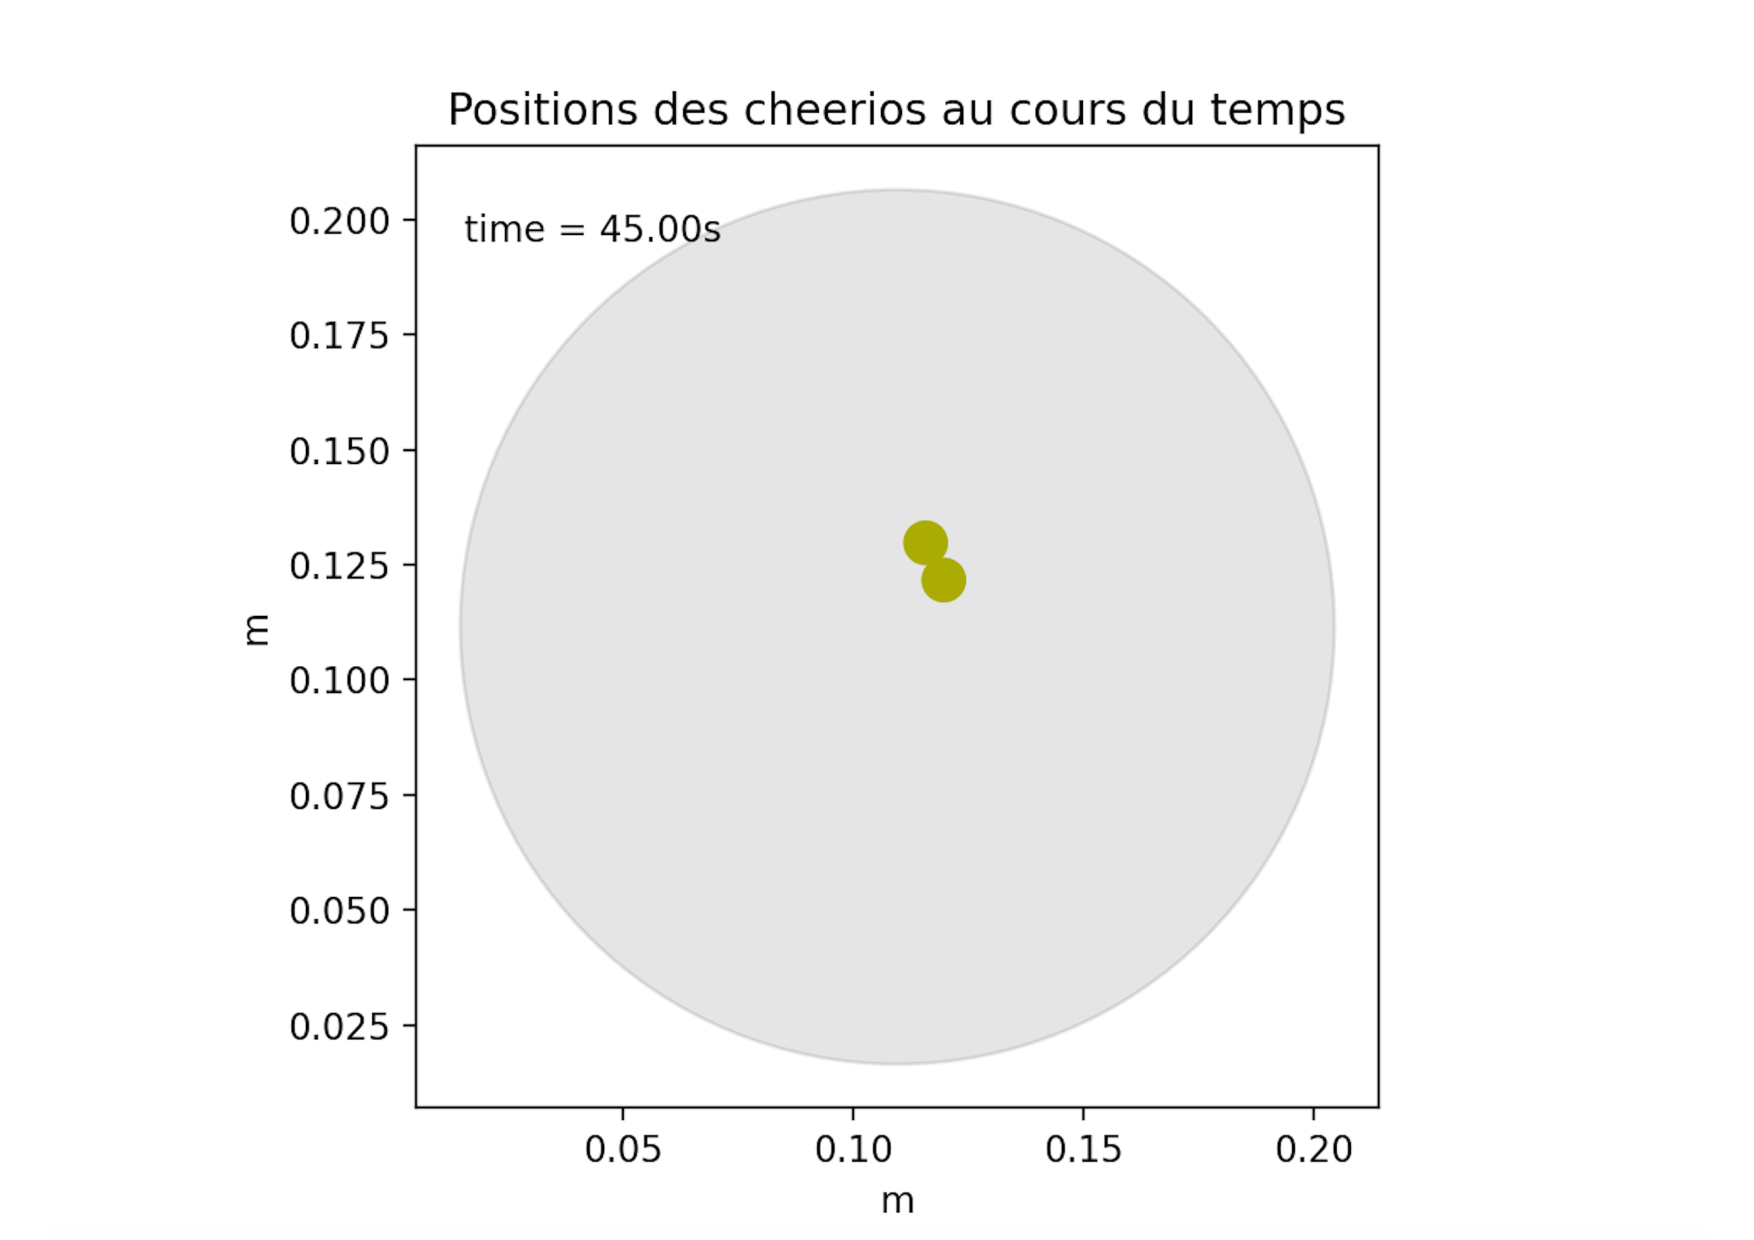
\includegraphics[width=0.4\textwidth, angle = 270]{visualisation3_1000_contact.pdf}
    %     \caption{Image de notre simulation lorsque les objets se touchent}
    %     \label{fig:simul_contact}
    % \end{figure}

    \begin{figure}%
        \centering
        \subfloat[\centering Simulation]{{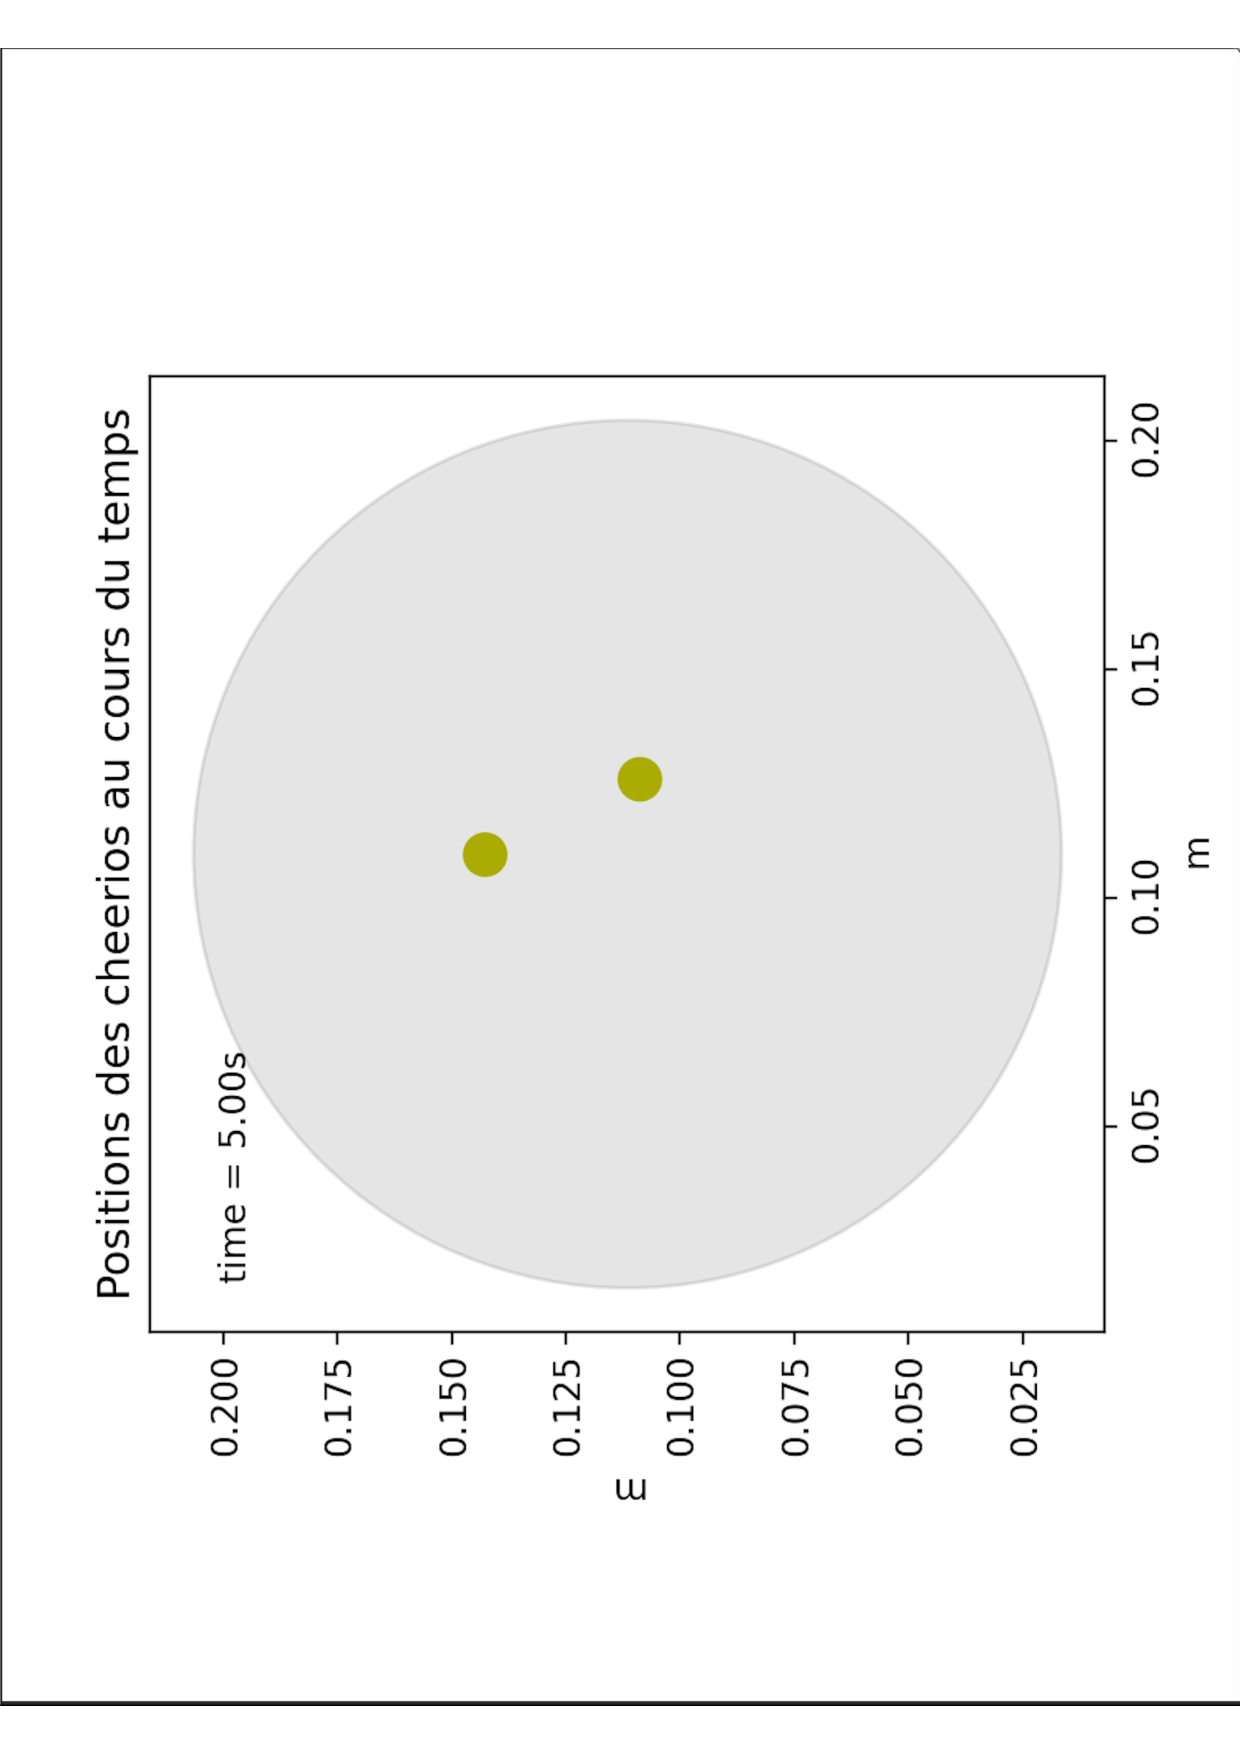
\includegraphics[height=5.5cm]{visualisation3_1000_init.pdf}}}%
        \qquad
        \subfloat[\centering Vraie vie]{{\includegraphics[width=5cm]{5sec.png}}}%
        \caption{A 5 secondes}%
        \label{fig:example}%
    \end{figure}
    % Ca marche ? non
    \begin{figure}%
        \centering
        \subfloat[\centering Simulation]{{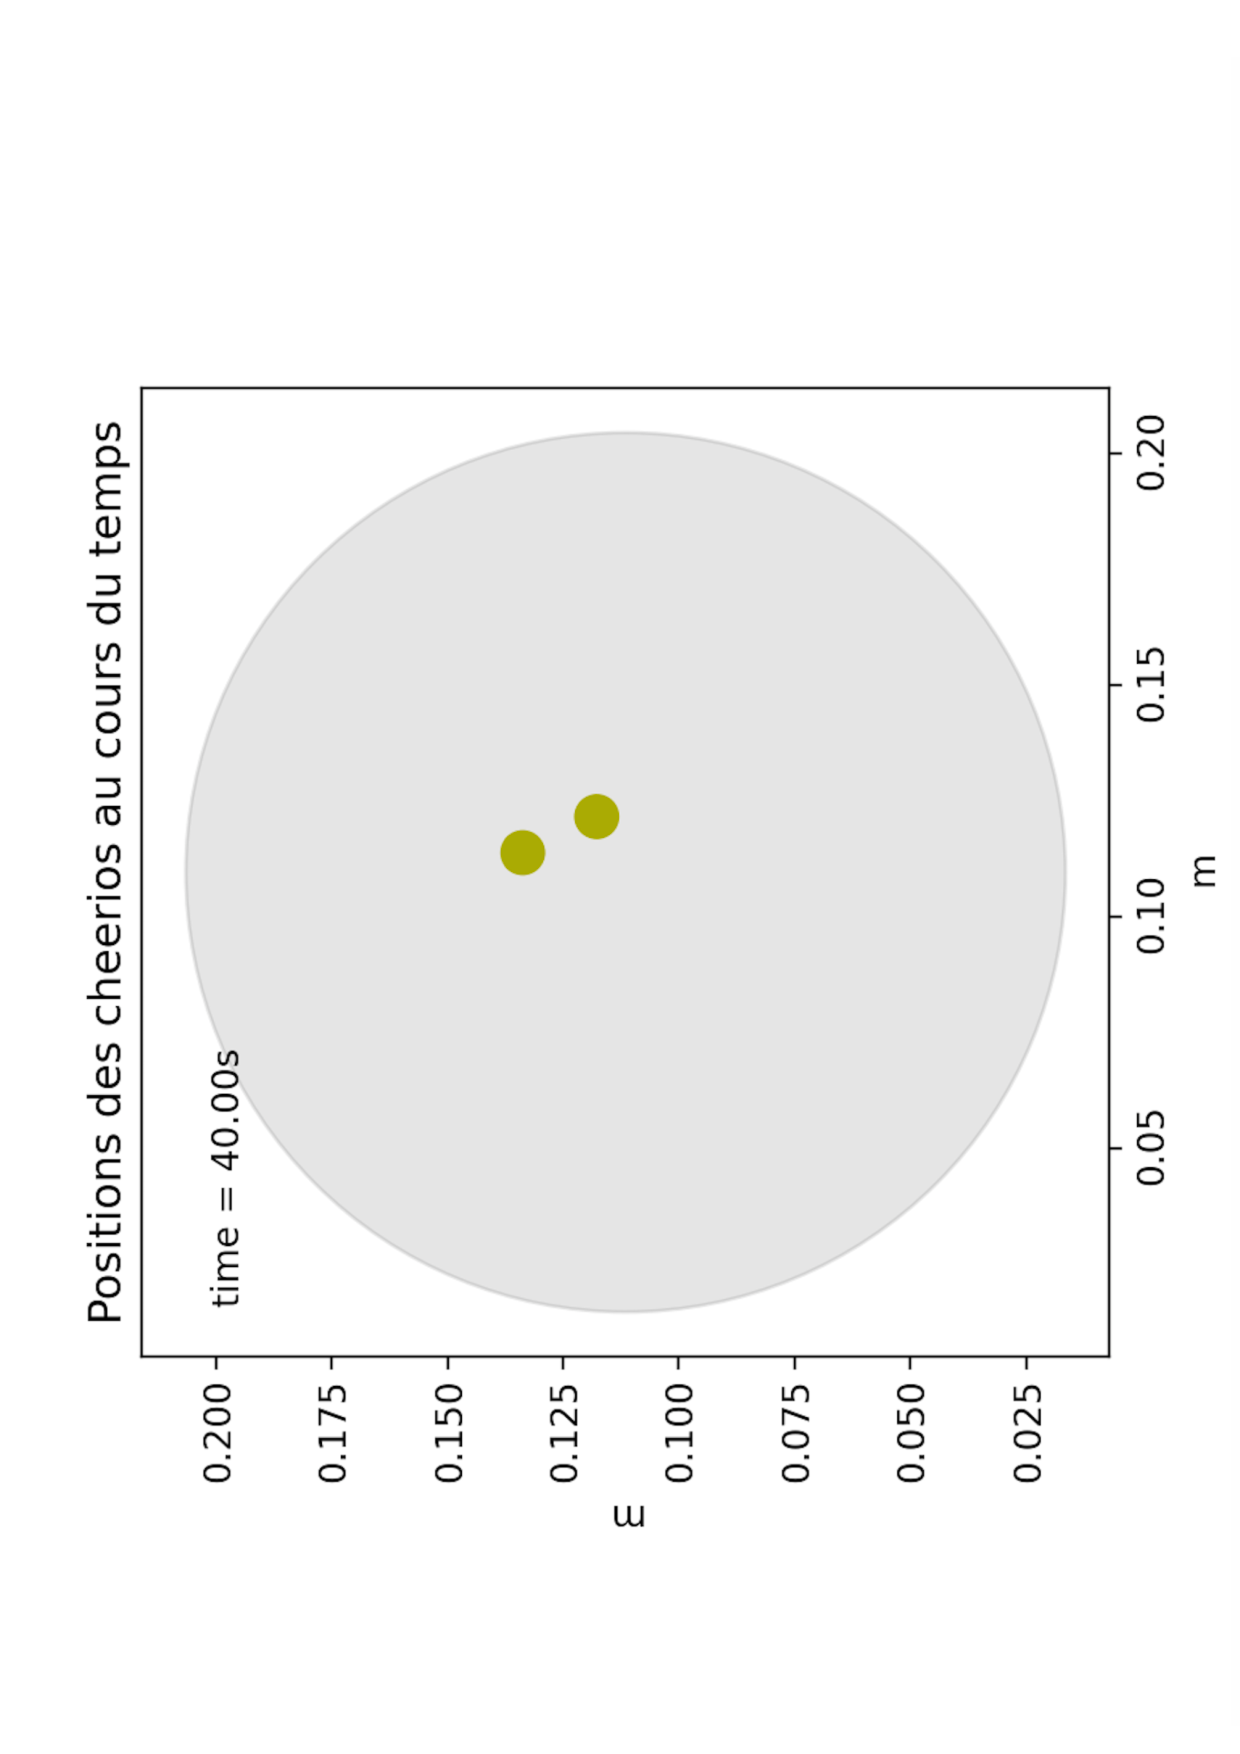
\includegraphics[height=5.5cm]{visualisation3_1000_pres.pdf}}}%
        \qquad
        \subfloat[\centering Vraie vie]{{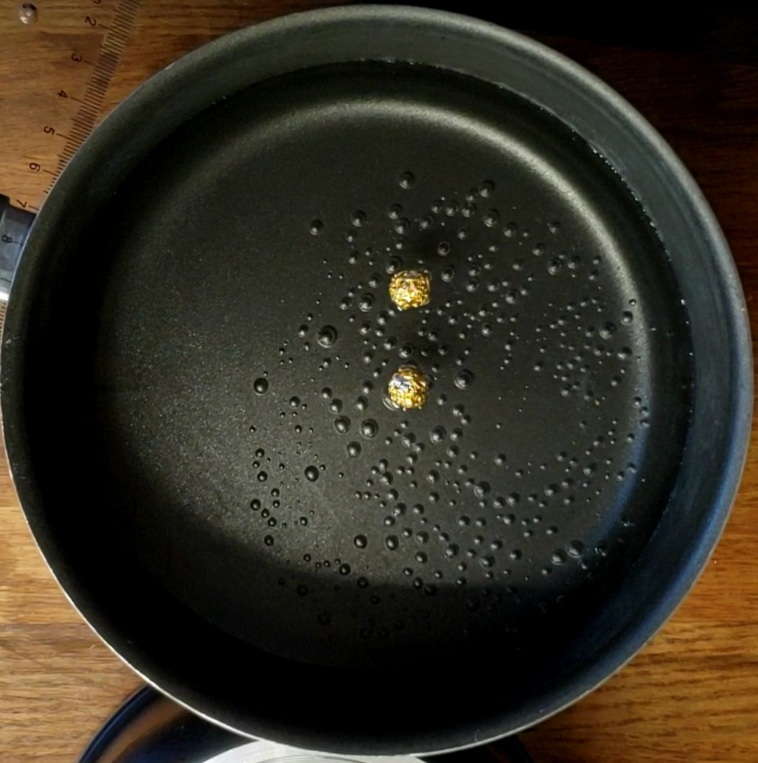
\includegraphics[width=5cm]{2eme.png}}}%
        \caption{A 40 secondes}%
        \label{fig:examplee}%
    \end{figure}
    \begin{figure}%
        \centering
        \subfloat[\centering Simulation]{{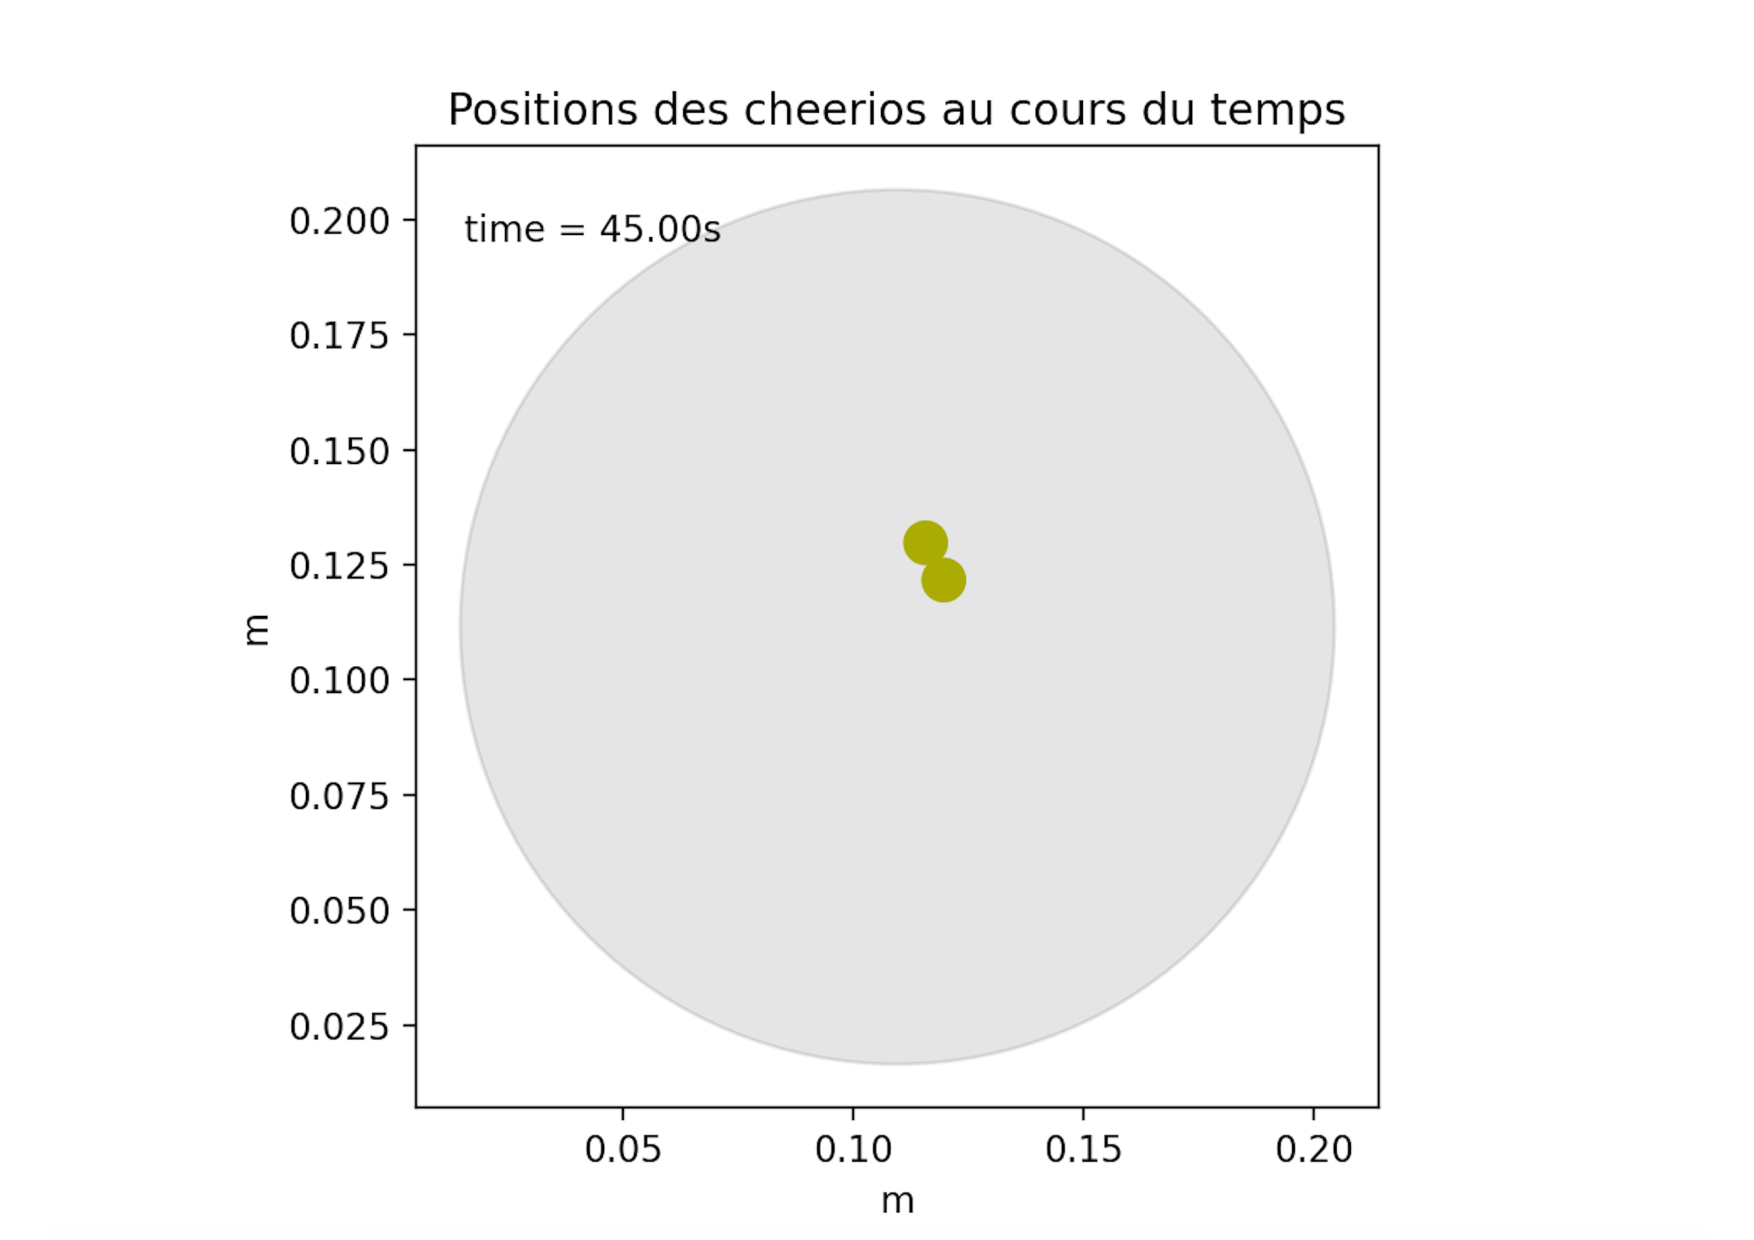
\includegraphics[height=5.5cm]{visualisation3_1000_contact.pdf}}}%
        \qquad
        \subfloat[\centering Vrai vie]{{\includegraphics[width=5cm]{45sec.png}}}%
        \caption{A 45 secondes}%
        \label{fig:examples}%
    \end{figure}
    
    Dans ces Figures, nous pouvons visualiser que la simulation n'est pas parfaite car il y a quelques différences avec les vidéos. L'une des raisons et que nous ne prenons pas en compte les légers écoulements d'air qu'il peut y avoir, qui ont des effets importants sur des objets flottants, de par leur faible stabilité. Néanmoins, nous pouvons être satisfait du résultat de nos simulations.
    
    %\includemovie{8cm}{6cm}{Figures/visualisationLongPrecis.gif}
\twocolumn
\section*{Conclusion}
    Pour conclure, nous avons réussi à analyser un problème de mécanique afin de créer une simulation de cet effet. Nous avons analysé le problème physique et l'avons résolu. Notre algorithme est fonctionnel et donne des résultats concluants. Cependant, notre code est fonctionnel jusqu'à une certaine durée. Après un certain temps la simulation devient instable. Néanmoins, nous avons su surpasser beaucoup de problème durant ce projet et nous avons pu développer nos techniques en programmation et notre savoir en mécanique des fluides, notamment avec notre recherche bibliographique qui eut une place importante dans ce projet. 
